% example.tex
%
% Copyright (C) 2010,2011 Laura Dietz
% Copyright (C) 2012 Jaakko Luttinen
%
% This file may be distributed and/or modified
%
% 1. under the LaTeX Project Public License and/or
% 2. under the GNU General Public License.
%
% See the files LICENSE_LPPL and LICENSE_GPL for more details.

\documentclass[a4paper]{article}

\usepackage{tikz}
\usetikzlibrary{bayesnet}
%\pgfrealjobname{example} % name of this file

\title{Graphical Models in Tikz}
\author{Laura Dietz, Jaakko Luttinen}

\begin{document}

\maketitle

TikZ examples for graphical models (Bayesian networks) and directed
factor graphs \cite{Dietz:2010}.

% A table of node types
\begin{table}[ht]
  \caption{Node types}
  \begin{center}
    \begin{tabular}{llc}
      Type & Syntax & Output
      \\
      \hline
      Latent variable &
      \texttt{\textbackslash node[latent]} &
      \tikz{ %
        \node[latent] {$x$}; %
      }
      \\
      Observed variable &
      \texttt{\textbackslash node[obs]} &
      \tikz{ %
        \node[obs] {$y$}; %
      }
      \\
      Deterministic &
      \texttt{\textbackslash node[det]} &
      \tikz{ %
        \node[det] {dot} ; %
      }
      \\
      Constant &
      \texttt{\textbackslash node[const]} &
      \tikz{ %
        \node[const] {$a$}; %
      }
      \\
      Factor &
      \texttt{\textbackslash node[factor]} &
      \tikz{ %
        \node[factor] [label=$\mathcal{N}$] {}; %
      }
    \end{tabular}
  \end{center}
\end{table}
\begin{table}[ht]
  \caption{Edge types}
  \begin{center}
    \begin{tabular}{llc}
      Type & Syntax & Output
      \\
      \hline
      Directed edges &
      \texttt{\textbackslash edge[opts]\{inputs\}\{outputs\}} &
      \tikz{ %
        \node[obs] (y) {$y$} ; %
        \node[latent, left=of y, yshift=0.5cm] (mu) {$\mu$} ; %
        \node[latent, left=of y, yshift=-0.5cm] (tau) {$\tau$} ; %
        \edge {mu,tau} {y} ; %
      }
      \\
      Undirected edges &
      \texttt{\textbackslash edge[-,opts]\{inputs\}\{outputs\}} &
      \tikz{ %
        \node[obs] (y) {$y$} ; %
        \node[latent, left=of y, yshift=0.5cm] (mu) {$\mu$} ; %
        \node[latent, left=of y, yshift=-0.5cm] (tau) {$\tau$} ; %
        \edge[-] {mu,tau} {y} ; %
      }
      \\
      Factor graph edges &
      \texttt{\textbackslash factoredge[opts]\{inputs\}\{via\}\{outputs\}} &
      \tikz{ %
        \node[obs] (y) {$y$} ; %
        \node[latent, left=of y, yshift=0.5cm] (mu) {$\mu$} ; %
        \node[latent, left=of y, yshift=-0.5cm] (tau) {$\tau$} ; %
        \factor[left=of y] {y-factor} {$\mathcal{N}$} {} {};
        \factoredge {mu,tau} {y-factor} {y} ; %
      }
    \end{tabular}
  \end{center}
\end{table}
\begin{table}[ht]
  \caption{Utilities}
  \begin{center}
    \begin{tabular}{llc}
      Type & Syntax & Output
      \\
      \hline
      Plate &
      \texttt{\textbackslash plate} &
      \tikz{ %
        \node[latent] (x) {$x_m$}; %
        \plate {} {(x)} {$m \in \mathcal{M}$}; %
      }
      \\
      Gate &
      &
      \tikz{
        % Nodes
        \node[obs]                    (k)   {$k$}; %
        \node[latent, above=2 of k]   (l)   {$\lambda$}; %
        \factor[above=0.8 of k]       {k-f} {Multi} {} {}; %
        \node[latent, right=of k-f]   (paa) {$\phi$}; %
        %\node[latent, right=of k-f]   (p)   {$\phi$}; %
        % Connections
        \factoredge {paa} {k-f} {k} ; %
        % Gate
        \gate {} {(k-f)(k-f-caption)} {l} ; %
      }
    \end{tabular}
  \end{center}
\end{table}


% Simple Bayesian network
\begin{figure}[ht]
  \begin{center}
    \begin{tabular}{cc}
      % model_pca.tex
%
% Copyright (C) 2012 Jaakko Luttinen
%
% This file may be distributed and/or modified
%
% 1. under the LaTeX Project Public License and/or
% 2. under the GNU General Public License.
%
% See the files LICENSE_LPPL and LICENSE_GPL for more details.

% PCA model

%\beginpgfgraphicnamed{model-pca}
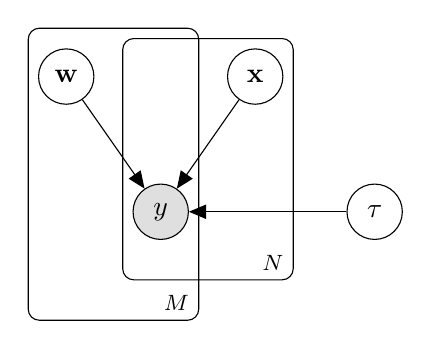
\begin{tikzpicture}

  % Define nodes
  \node[obs]                               (y) {$y$};
  \node[latent, above=of y, xshift=-1.2cm] (w) {$\mathbf{w}$};
  \node[latent, above=of y, xshift=1.2cm]  (x) {$\mathbf{x}$};
  \node[latent, right=2cm of y]            (t) {$\tau$};

  % Connect the nodes
  \edge {x,w,t} {y} ; %

  % Plates
  \plate {yx} {(x)(y)} {$N$} ;
  \plate {} {(w)(y)(yx.north west)(yx.south west)} {$M$} ;

\end{tikzpicture}
%\endpgfgraphicnamed

%%% Local Variables: 
%%% mode: tex-pdf
%%% TeX-master: "example"
%%% End: 
 &
      % model_pca2.tex
%
% Copyright (C) 2010,2011 Laura Dietz
% Copyright (C) 2012 Jaakko Luttinen
%
% This file may be distributed and/or modified
%
% 1. under the LaTeX Project Public License and/or
% 2. under the GNU General Public License.
%
% See the files LICENSE_LPPL and LICENSE_GPL for more details.

% PCA model

%\beginpgfgraphicnamed{model-pca}
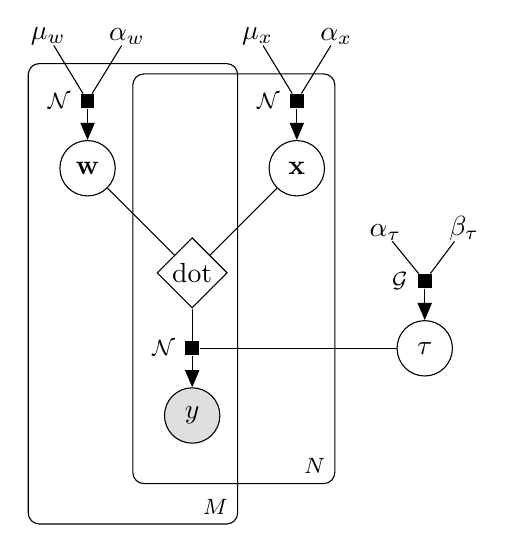
\begin{tikzpicture}

  % Define nodes

  % Y
  \node[obs]          (y)   {$y$}; %
  \factor[above=of y] {y-f} {left:$\mathcal{N}$} {} {} ; %

  % W and X
  \node[det, above=of y]            (dot) {dot} ; % 
  \node[latent, above left=1.2 of dot]  (w)   {$\mathbf{w}$}; %
  \node[latent, above right=1.2 of dot] (x)   {$\mathbf{x}$}; %

  % W hyperparameters
  \node[const, above=1.2 of w, xshift=-0.5cm] (mw) {$\mu_w$} ; %
  \node[const, above=1.2 of w, xshift=0.5cm]  (aw) {$\alpha_w$} ; %

  % X hyperparameters
  \node[const, above=1.2 of x, xshift=-0.5cm] (mx) {$\mu_x$} ; %
  \node[const, above=1.2 of x, xshift=0.5cm]  (ax) {$\alpha_x$} ; %

  % noise
  \node[latent, right=2.5cm of y-f]         (t)   {$\tau$}; %
  \node[const, above=of t, xshift=-0.5cm] (at)  {$\alpha_\tau$} ; %
  \node[const, above=of t, xshift=0.5cm]  (bt)  {$\beta_\tau$} ; %

  % Factors
  \factor[above=of w] {w-f} {left:$\mathcal{N}$} {mw,aw} {w} ; %
  \factor[above=of x] {x-f} {left:$\mathcal{N}$} {mx,ax} {x} ; %
  \factor[above=of t] {t-f} {left:$\mathcal{G}$} {at,bt} {t} ; %
  \factoredge {dot,t} {y-f} {y} ; %

  % Connect w and x to the dot node
  \edge[-] {w,x} {dot} ;

  % Plates
  \plate {yx} { %
    (y)(y-f)(y-f-caption) %
    (x)(x-f)(x-f-caption) %
    (dot) %
  } {$N$} ;
  \plate {} {%
    (y)(y-f)(y-f-caption) %
    (w)(w-f)(w-f-caption) %
    (dot) %
    (yx.north west)(yx.south west) %
  } {$M$} ;

\end{tikzpicture}
%\endpgfgraphicnamed

%%% Local Variables: 
%%% mode: tex-pdf
%%% TeX-master: "example"
%%% End: 


    \end{tabular}
  \end{center}
  \caption{PCA model as a Bayesian network and a directed factor
    graph.}
\end{figure}

% Latent Dirichlet allocation
\begin{figure}[ht]
  \begin{center}
    % model_lda.tex
%
% Copyright (C) 2010,2011 Laura Dietz
% Copyright (C) 2012 Jaakko Luttinen
%
% This file may be distributed and/or modified
%
% 1. under the LaTeX Project Public License and/or
% 2. under the GNU General Public License.
%
% See the files LICENSE_LPPL and LICENSE_GPL for more details.

% Latent Diriclet allocation model

%\beginpgfgraphicnamed{model-lda}
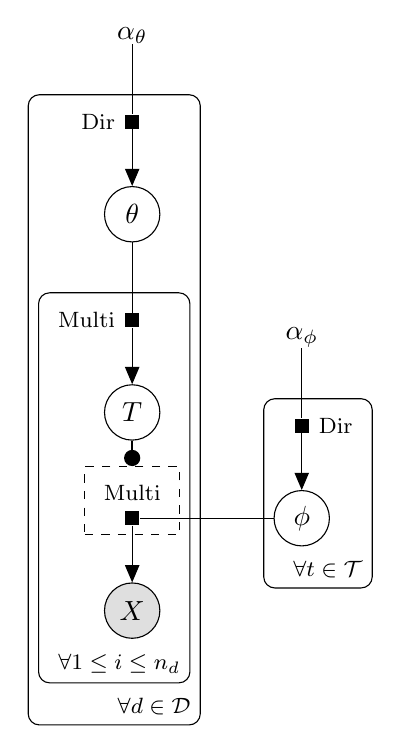
\begin{tikzpicture}[x=1.7cm,y=1.8cm]

  % Nodes

  \node[obs]                   (X)      {$X$} ; %
  \node[latent, above=of X]    (T)      {$T$} ; %
  \node[latent, above=of T]    (theta)  {$\theta$}; %
  \node[const, above=of theta] (atheta) {$\alpha_\theta$};


  % Factors
  \factor[above=of X]     {X-f}     {Multi} {} {} ; %
  \factor[above=of T]     {T-f}     {left:Multi} {} {} ; %
  \factor[above=of theta] {theta-f} {left:Dir} {} {} ; %

  % More nodes
  \node[latent, right=of X-f] (phi)  {$\phi$}; %
  \node[const, above=of phi]  (aphi) {$\alpha_\phi$}; %

  \factor[above=of phi] {phi-f} {right:Dir} {} {} ; %

  \factoredge {theta}  {T-f}     {T} ; %
  \factoredge {atheta} {theta-f} {theta} ; %
  \factoredge {phi}    {X-f}     {X} ; %
  \factoredge {aphi}   {phi-f}   {phi} ; %

  \gate {X-gate} {(X-f)(X-f-caption)} {T}

  \plate {plate1} { %
    (X)(X-gate) %
    (T)(T-f)(T-f-caption) %
  } {$\forall 1 \leq i \leq n_d$}; %
  \plate {} { %
    (plate1) %
    (theta)(theta-f)(theta-f-caption) %
  } {$\forall d \in \mathcal{D}$} ; %
  \plate {} { %
    (phi)(phi-f)(phi-f-caption) %
  } {$\forall t \in \mathcal{T}$} ; %

\end{tikzpicture}
%\endpgfgraphicnamed

%%% Local Variables: 
%%% mode: tex-pdf
%%% TeX-master: "example"
%%% End: 

  \end{center}
  \caption{Latent Dirichlet allocation as directed factor graph.}
\end{figure}

% Citation influence model
\begin{figure}[ht]
  \begin{center}
    % model_citation_influence.tex
%
% Copyright (C) 2010,2011 Laura Dietz
% Copyright (C) 2012 Jaakko Luttinen
%
% This file may be distributed and/or modified
%
% 1. under the LaTeX Project Public License and/or
% 2. under the GNU General Public License.
%
% See the files LICENSE_LPPL and LICENSE_GPL for more details.

% Citation influence model
% Cite this model as 
% Laura Dietz, Steffen Bickel, Tobias Scheffer. 
% Unsupervised Prediction of Citation Influences. 
% In: Proceedings of International Conference on Machine Learning. 2007

%\beginpgfgraphicnamed{model-citation-influence}
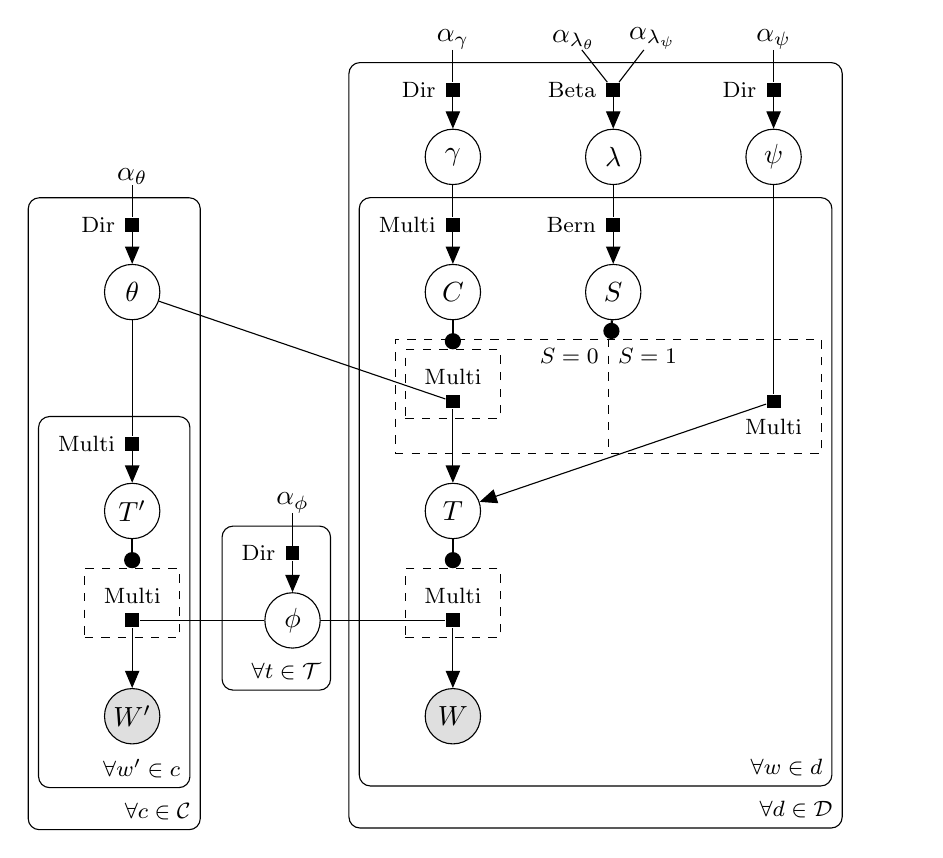
\begin{tikzpicture}

  % Layout the variables
  \matrix[row sep=0.5cm, column sep=1.2cm] (LDA)
  { %
    & %
    & %
    \node[latent] (gamma)  {$\gamma$} ; & %
    \node[latent] (lambda) {$\lambda$} ; & %
    \node[latent] (psi)    {$\psi$} ; %
    \\
    \\
    \node[latent] (theta)  {$\theta$} ; & %
    & %
    \node[latent] (C)      {$C$} ; & %
    \node[latent] (S)      {$S$} ; & %
    \\
    & %
    & %
    \factor       {T-f1}   {Multi} {} {}; & %
    & %
    \factor       {T-f2}   {below:Multi} {} {}; & %
    \\
    \node[latent] (T')     {$T'$} ; & %
    & %
    \node[latent] (T)      {$T$} ; & %
    \\
    \factor       {W'-f}   {Multi} {} {}; & %
    \node[latent] (phi)    {$\phi$} ; & %
    \factor       {W-f}    {Multi} {} {}; %
    \\
    \node[obs] (W')        {$W'$} ; & %
    & %
    \node[obs] (W)         {$W$} ;
    \\
  };

  % Remaining factors
  \factor[above=of T']     {T'-f}     {left:Multi} {} {}; %
  \factor[above=of theta]  {theta-f}  {left:Dir} {} {}; %
  \factor[above=of C]      {C-f}      {left:Multi} {} {}; %
  \factor[above=of S]      {S-f}      {left:Bern} {} {}; %
  \factor[above=of gamma]  {gamma-f}  {left:Dir} {} {}; %
  \factor[above=of lambda] {lambda-f} {left:Beta} {} {}; %
  \factor[above=of psi]    {psi-f}    {left:Dir} {} {}; %
  \factor[above=of phi]    {phi-f}    {left:Dir} {} {}; %

  % Hyperparameters
  \node[const, above=of theta]  (atheta)  {$\alpha_\theta$}; %
  \node[const, above=of phi]    (aphi)    {$\alpha_\phi$}; %
  \node[const, above=of gamma]  (agamma)  {$\alpha_\gamma$}; %
  \node[const, above=of lambda, xshift=-0.5cm] (alambda1)
  {$\alpha_{\lambda_\theta}$}; %
  \node[const, above=of lambda, xshift=0.5cm] (alambda2)
  {$\alpha_{\lambda_\psi}$}; %
  \node[const, above=of psi]    (apsi)    {$\alpha_\psi$}; %

  % Factor connections
  \factoredge {phi}               {W'-f}     {W'} ; %
  \factoredge {phi}               {W-f}      {W} ; %
  \factoredge {theta}             {T'-f}     {T'} ; %
  \factoredge {theta}             {T-f1}     {T} ; %
  \factoredge {psi}               {T-f2}     {T} ; %
  \factoredge {atheta}            {theta-f}  {theta} ; %
  \factoredge {gamma}             {C-f}      {C} ; %
  \factoredge {lambda}            {S-f}      {S} ; %
  \factoredge {agamma}            {gamma-f}  {gamma} ; %
  \factoredge {alambda1,alambda2} {lambda-f} {lambda} ; %
  \factoredge {apsi}              {psi-f}    {psi} ; %
  \factoredge {aphi}              {phi-f}    {phi} ; %

  % Gates
  \gate {W'-gate} {(W'-f)(W'-f-caption)} {T'} ; %
  \gate {W-gate}  {(W-f)(W-f-caption)}   {T} ; %
  \gate {T-gate}  {(T-f1)(T-f1-caption)} {C} ;
  \vgate {T-vgate} %
  {(T-gate)} {$S=0$} %
  {(T-f2)(T-f2-caption)} {$S=1$} %
  {S} ; %

  % Plates
  \plate {LDA1} { %
    (T')(T'-f)(T'-f-caption) %
    (W')(W'-gate) %
  } {$\forall w' \in c$} ; %

  \plate {LDA2} { %
    (LDA1) %
    (theta)(theta-f)(theta-f-caption) %
  } {$\forall c \in \mathcal{C}$} ; %

  \plate {} { %
    (phi)(phi-f)(phi-f-caption) %
  } {$\forall t \in \mathcal{T}$} ; %

  \plate {P1} { %
    (W)(W-gate) %
    (T)(T-vgate) %
    (C)(C-f)(C-f-caption) %
    (S)(S-f)(S-f-caption) %
  } {$\forall w \in d$} ;

  \plate {} { %
    (P1) %
    (gamma)(gamma-f)(gamma-f-caption) %
    (lambda)(lambda-f)(lambda-f-caption) %
    (psi)(psi-f)(psi-f-caption) %
  } {$\forall d \in \mathcal{D}$} ; %

\end{tikzpicture}
%\endpgfgraphicnamed

%%% Local Variables: 
%%% mode: tex-pdf
%%% TeX-master: "example"
%%% End: 

  \end{center}
  \caption{Citation influence model with own topics \cite{Dietz:2007}
    as directed factor graph.}
\end{figure}

\clearpage

\begin{thebibliography}{9}

\bibitem{Dietz:2010}
  Laura Dietz,
  \emph{Directed Factor Graph Notation for Generative Models}.
  Technical Report. 2010

% Laura Dietz, Steffen Bickel, Tobias Scheffer. 
% Unsupervised Prediction of Citation Influences. 
% In: Proceedings of International Conference on Machine Learning. 2007
\bibitem{Dietz:2007}
  Laura Dietz, Steffen Bickel, Tobias Scheffer,
  \emph{Unsupervised Prediction of Citation Influences}.
  In: Proceedings of International Conference on Machine
  Learning. 2007


\end{thebibliography}

\end{document}

%%% Local Variables: 
%%% mode: tex-pdf
%%% TeX-master: t
%%% End: 
